\begin{figure}
	\centering
%	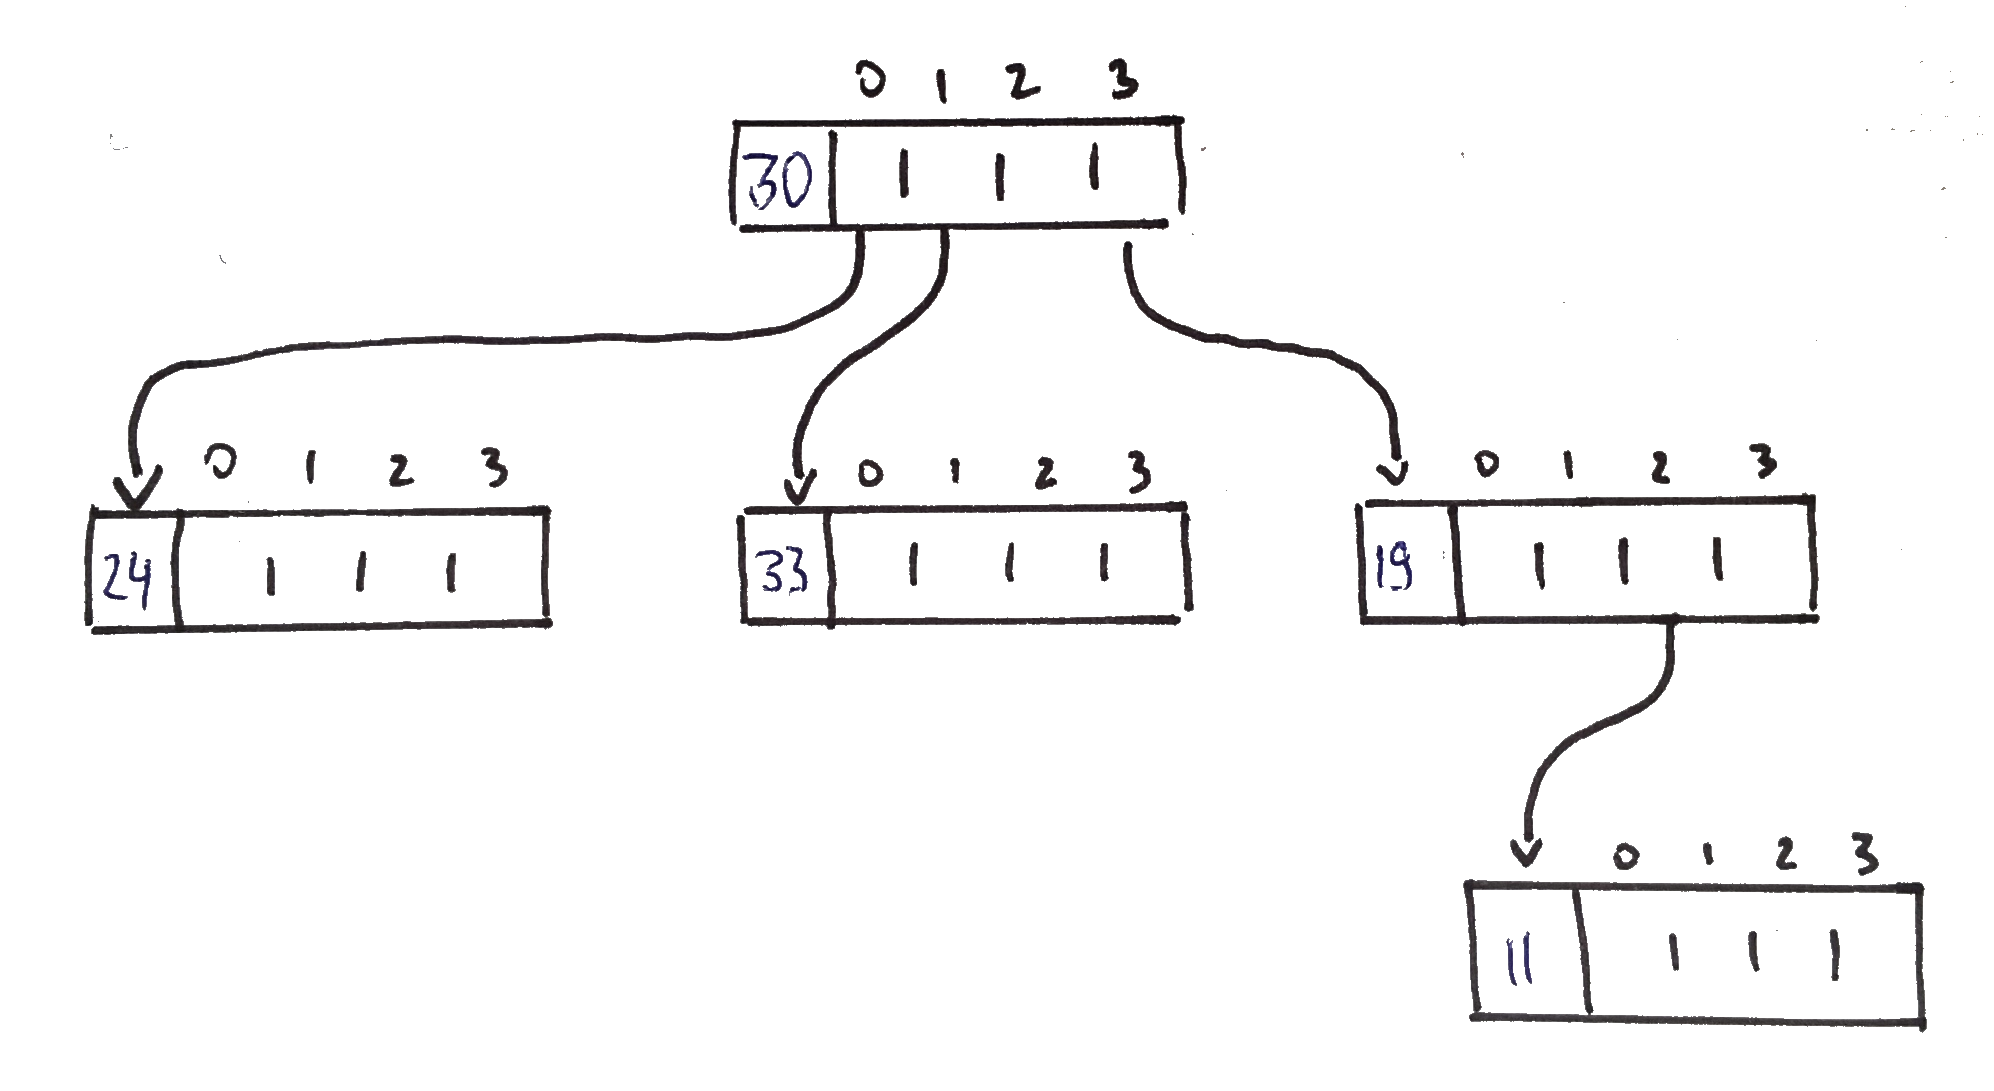
\includegraphics[width=\textwidth]{topic/imgtries/sampletrie_drawn_transp}
	\newcommand{\trienode}[2]{% node label, options for matrix
	\matrix (n#1) [table, text width=7mm, ampersand replacement=\&, #2]
	{ #1 \& {} \& {} \& {} \& {} \\};
	\node[font=\tiny, anchor=south] at (n#1-1-2.north) {0};
	\node[font=\tiny, anchor=south] at (n#1-1-3.north) {1};
	\node[font=\tiny, anchor=south] at (n#1-1-4.north) {2};
	\node[font=\tiny, anchor=south] at (n#1-1-5.north) {3}
}

\begin{tikzpicture}[align=center, node distance=2.5cm]
	\trienode{30}{};	
	\trienode{33}{below of=n30};
	\trienode{24}{left =2cm of n33};
	\trienode{19}{right=2cm of n33};
	\trienode{11}{below of=n19};
	
	\trienode{45}{below of=n33, dashed};
	
	\draw[edge] (n30-1-2) to[out=270, in=90] (n24-1-1.north);
	\draw[edge] (n30-1-3.south) to[out=270, in=90] (n33-1-1.north);
	\draw[edge] (n30-1-5.south) to[out=270, in=90] (n19-1-1.north);
	\draw[edge] (n19-1-4.south) to[out=270, in=90] (n11-1-1.north);
	
	\draw[edge, dashed] (n33-1-5.south) to[out=270, in=90] (n45-1-1.north);
\end{tikzpicture}
	\caption{ \small A trie with $k = 4$ and entries 30, 24, 33, 19 and 11.
		To insert 45, we repeatedly divide 45 by 4, giving
			$45 \overset{1}{\longrightarrow} 11  \overset{3}{\longrightarrow} 2$.
		The remainders 1 and 3 lead to 33 where we insert a new node at slot 3 with value 45 as indicated.
		To delete 19, we search for it with the sequence $19 \overset{3}{\longrightarrow} 4$.
		Then, we localise a leaf that is a descendant of 19, in this trie, only 11 is possible.
		We remove 11 and set the value of 19 to 11.
		\label{fig:trie}}
\end{figure}


A trie \cite{knuth:tries} is a data structure.
In fact, a trie is a tree with the same maximum branching factor $k$ for all nodes.
A trie differs from balanced binary trees or other types of trees in the way that elements are inserted, looked up and deleted.
Every node of a trie contains an integer and $k$ pointers to its child nodes, indexed from 0 through $k - 1$.
Typically, $k$ is a power of 2.
The pointers in every node are \emph{null} initially and may be set when new elements are added.
The first element that is added to an empty trie is stored in the root and no new nodes are created.
Subsequent elements are added as follows:
Given a new element $e$, we repeatedly divide $e$ by $k$.
This gives a sequence of quotients and remainders.
Since the remainders are in the range 0 through $k - 1$, they specify a sequence of pointers.
The sequence starts at the root and descends one level into the tree with every step.
We follow the sequence of pointers until we reach a null pointer, which is where we insert a new node with value $e$.
This completes the insertion of a value into a trie.
Searching a value $v$ in a trie happens in a similar way:
First, we check for $v$ in the root.
If $v$ is not present there, we follow the sequence of remainders as above.
At every node, we check if it contains $v$.
If we eventually reach a null pointer the trie does not contain $v$, otherwise it does.
To delete a value $u$, we first search for $u$ in the trie and store the node $n_u$ which contains $u$.
If $n_u$ is a leaf, we simply delete it.
Otherwise, we locate any leaf that is a descendant of $n_u$, replace the value in $n_u$ by the leaf's value and then remove the leaf from the trie.
Examples for the operations can be found in Figure~\ref{fig:trie}.
A trie requires $\O{kn}$ space in the worst case.
The longest path starting at the root node in a trie has length $\O{\log_k\pfrac{N}{n}}$.
This means that search, insertion and deletion in a trie have the same time complexity:
During each operation, we follow some path in the trie.
In the worst case, the path is the longest in the trie and we follow it until we reach a leaf which requires $\O{\log_k\pfrac{N}{n}}$ time.
Insertion and deletion additionally manipulate some nodes, but in both cases these changes are constant time because only one or two nodes must be changed.
If the values to be inserted into a trie are uniformly and independently distributed, lookup and insertion time are $\O{1}$.
